
\begin{exercise}
  State a score theorem for weighted graphs when we allow
  negative edge weights. That is, state a theorem like
  \begin{theorem}[Score Theorem for Graphs with Real Edge Weights]
     Let $(a_1,\dots,a_n) \in \R^n$. There is a  graph with real edge weights
     with this score if and only if $n \geq 3$ or $a_1 = a_2$ when $n=2$ or $a_1 = 0$ when $n=1$.
  \end{theorem}  
\end{exercise}

\begin{exercise}
Prove your theorem.
    \begin{proof}

        Obviously, if there is a graph with real edge weights, $n \geq 3$ or $a_1 = a_2$ when $n=2$ or $a_1 = 0$ when $n=1$.

        Suppose $v_1, v_2 , \dots, v_n$ are the corresponding vertices of $a_1, a_2, \dots, a_n$.

        When $n=1$, obviously, there is a graph with real edge weights if and only if $a_1=0$.

        When $n=2$, obviously, there is a graph with real edge weights if and only if $a_1=a_2$.

        When $n=3$, suppose $x, y, z$ be the weight of $E(v_2, v_3), E(v_1, v_3), E(v_1, v_2)$.

        According to the degree of each vertices, there are equations as followings:
        $$
        \begin{cases}
            x + y = a_3 \\
            x + z = a_2 \\
            y + z = a_1
        \end{cases}
        $$

        The solution is:
        $$
        \begin{cases}
            x = \frac{a_2 + a_3 - a_1}{2} \\
            y = \frac{a_1 + a_3 - a_2}{2} \\
            z = \frac{a_1 + a_2 - a_3}{2}
        \end{cases}
        $$

        Therefore, for every sequence $a_1, a_2, a_3$, there is a graph with real edge weights.

        When $n \geq 4$.

        Connect an edge of weight $a_i$ between $v_i$ and $v_1$, $i \geq 4$.

        Now we can image $v_1, v_4, \dots, v_n$ as a "big" vertice $v_1^\prime$. To promise the degree of $v_1$, the degree of the "big" vertice is $a_1^\prime = a_1 - a_4 - \dots - a_n$.

        In fact, it becomes the cases that $n=3$.
        Suppose $x, y, z$ be the weight of $E(v_2, v_3), E(v_1^\prime, v_3), E(v_1^\prime, v_2)$.

        $$
        \begin{cases}
            x + y = a_3 \\
            x + z = a_2 \\
            y + z = a_1^\prime
        \end{cases}
        $$

        $$
        \begin{cases}
            x = \frac{a_2 + a_3 - a_1^\prime}{2} \\
            y = \frac{a_1^\prime + a_3 - a_2}{2} \\
            z = \frac{a_1^\prime + a_2 - a_3}{2}
        \end{cases}
        $$

\begin{center}
  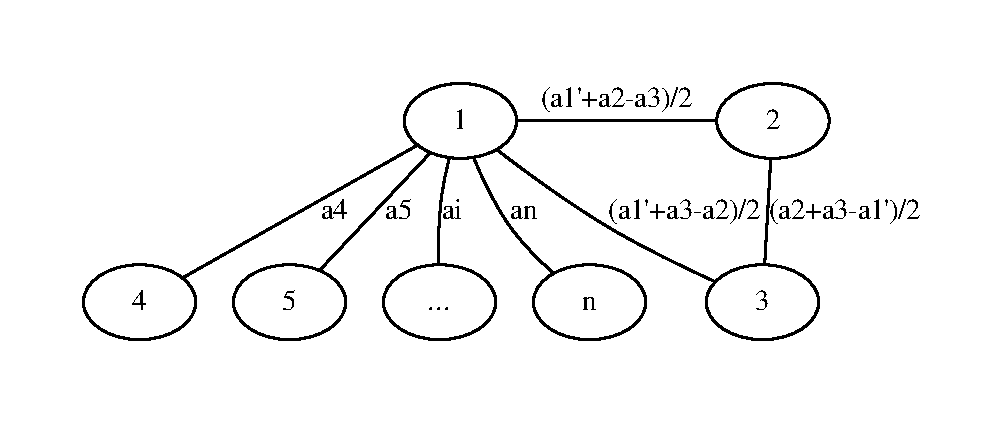
\includegraphics[width=0.5\textwidth]{figures/7-8.pdf}
\end{center}

    Therefore, for $a_1, a_2, \dots, a_n$, $n \geq 4$, there is a graph with real edge weight.

    \end{proof}
\end{exercise}

